%%%% ijcai16.tex

\typeout{Constructive Preference Elicitation by Setwise Max-margin Learning}

\documentclass{article}
\usepackage{ijcai16}
\usepackage{graphicx}
\usepackage{times}
%\usepackage{latexsym}

\RequirePackage{amsmath,amssymb,amsfonts,amsthm}
\usepackage{algorithm}
\usepackage{algpseudocode}

% ---------------------------------------------------------------------------

\algrenewcommand{\algorithmicrequire}{\textbf{Input:}}
\algrenewcommand{\algorithmicensure}{\textbf{Output:}}

\renewcommand\[{\begin{equation}}
\renewcommand\]{\end{equation}}

% Bold math symbols
\newcommand{\bbA}{\mathbb{A}}
\newcommand{\bbB}{\mathbb{B}}
\newcommand{\bbC}{\mathbb{C}}
\newcommand{\bbD}{\mathbb{D}}
\newcommand{\bbE}{\mathbb{E}}
\newcommand{\bbF}{\mathbb{F}}
\newcommand{\bbG}{\mathbb{G}}
\newcommand{\bbH}{\mathbb{H}}
\newcommand{\bbI}{\mathbb{I}}
\newcommand{\bbJ}{\mathbb{J}}
\newcommand{\bbK}{\mathbb{K}}
\newcommand{\bbL}{\mathbb{L}}
\newcommand{\bbM}{\mathbb{M}}
\newcommand{\bbN}{\mathbb{N}}
\newcommand{\bbO}{\mathbb{O}}
\newcommand{\bbP}{\mathbb{P}}
\newcommand{\bbQ}{\mathbb{Q}}
\newcommand{\bbR}{\mathbb{R}}
\newcommand{\bbS}{\mathbb{S}}
\newcommand{\bbT}{\mathbb{T}}
\newcommand{\bbU}{\mathbb{U}}
\newcommand{\bbV}{\mathbb{V}}
\newcommand{\bbW}{\mathbb{W}}
\newcommand{\bbX}{\mathbb{X}}
\newcommand{\bbY}{\mathbb{Y}}
\newcommand{\bbZ}{\mathbb{Z}}

% Calligraphic math symbols
\newcommand{\calvar}[1]{\ensuremath{\mathcal{#1}}}
\newcommand{\calA}{\calvar{A}}
\newcommand{\calB}{\calvar{B}}
\newcommand{\calC}{\calvar{C}}
\newcommand{\calD}{\calvar{D}}
\newcommand{\calE}{\calvar{E}}
\newcommand{\calF}{\calvar{F}}
\newcommand{\calG}{\calvar{G}}
\newcommand{\calH}{\calvar{H}}
\newcommand{\calI}{\calvar{I}}
\newcommand{\calJ}{\calvar{J}}
\newcommand{\calK}{\calvar{K}}
\newcommand{\calL}{\calvar{L}}
\newcommand{\calM}{\calvar{M}}
\newcommand{\calN}{\calvar{N}}
\newcommand{\calO}{\calvar{O}}
\newcommand{\calP}{\calvar{P}}
\newcommand{\calQ}{\calvar{Q}}
\newcommand{\calR}{\calvar{R}}
\newcommand{\calS}{\calvar{S}}
\newcommand{\calT}{\calvar{T}}
\newcommand{\calU}{\calvar{U}}
\newcommand{\calV}{\calvar{V}}
\newcommand{\calW}{\calvar{W}}
\newcommand{\calX}{\calvar{X}}
\newcommand{\calY}{\calvar{Y}}
\newcommand{\calZ}{\calvar{Z}}

% Vectors
\newcommand{\vecvar}[1]{\ensuremath{\boldsymbol{#1}}}
\newcommand{\va}{\vecvar{a}}
\newcommand{\vb}{\vecvar{b}}
\newcommand{\vc}{\vecvar{c}}
\newcommand{\vd}{\vecvar{d}}
\newcommand{\ve}{\vecvar{e}}
\newcommand{\vf}{\vecvar{f}}
\newcommand{\vg}{\vecvar{g}}
\newcommand{\vh}{\vecvar{h}}
\newcommand{\vi}{\vecvar{i}}
\newcommand{\vj}{\vecvar{j}}
\newcommand{\vk}{\vecvar{k}}
\newcommand{\vl}{\vecvar{l}}
\newcommand{\vm}{\vecvar{m}}
\newcommand{\vn}{\vecvar{n}}
\newcommand{\vo}{\vecvar{o}}
\newcommand{\vp}{\vecvar{p}}
\newcommand{\vq}{\vecvar{q}}
\newcommand{\vr}{\vecvar{r}}
\newcommand{\vs}{\vecvar{s}}
\newcommand{\vt}{\vecvar{t}}
\newcommand{\vu}{\vecvar{u}}
\newcommand{\vv}{\vecvar{v}}
\newcommand{\vw}{\vecvar{w}}
\newcommand{\vx}{\vecvar{x}}
\newcommand{\vy}{\vecvar{y}}
\newcommand{\vz}{\vecvar{z}}
\newcommand{\valpha}{\vecvar{\alpha}}
\newcommand{\veps}{\vecvar{\varepsilon}}
\newcommand{\vphi}{\vecvar{\varphi}}
\newcommand{\vpsi}{\vecvar{\psi}}
\newcommand{\vtheta}{\vecvar{\theta}}

% Operators
\DeclareMathOperator*{\argmax}{argmax}
\DeclareMathOperator*{\argmin}{argmin}

% Debugging

\usepackage{color}
\newcommand{\andrea}[1]{{\bf \textcolor{blue}{{\fbox{Andrea:} #1}}}}
\newcommand{\stefano}[1]{{\bf \textcolor{green}{{\fbox{Stefano:} #1}}}}
\newcommand{\paolo}[1]{{\bf \textcolor{red}{{\fbox{Paolo:} #1}}}}

% ---------------------------------------------------------------------------

\title{Constructive Preference Elicitation by Setwise Max-margin Learning}
\author{ST and AP and PV}

\begin{document}

\maketitle

\begin{abstract}
WRITEME
\end{abstract}

\section{Introduction}

WRITEME

- importance of recommendation systems and preference elicitation

- existing approaches and their limitations

% constructive preference elicitation
In this paper we take a {\em constructive} view on preference
elicitation, enlarging its scope from the selection of items among a
set of candidates to the synthesis of entirely novel
instances. Instances are represented as combinations of basic elements
(e.g. the components of a laptop) subject to a set of constraints
(e.g. the laptop model determines the set of available CPUs). A
utility function is learned over the feature representation of an
instance, as customary in many preference elicitation approaches. The
recommendation is then made by solving a constrained optimization
problem in the space of feasible instances, guided by the learned
utility. \andrea{other constructive preference elicitation approaches?}

% setwise max-margin formulation to deal with uncertainty in user utility
Learning a user utility function requires setting a preference
elicitation strategy and dealing with uncertain and possibly
inconsistent user feedback. Bayesian preference elicitation approaches
deal with both problems by building a probability distribution on
candidate functions and asking queries maximizing informativeness
measures such as expected value of information (EVOI)~\cite{}. These
approaches are however computationally expensive and cannot scale to
fully constructive scenarios, as shown in our experimental results.
We take a space decomposition perspective and jointly learn a set of
weight vectors, each representing a candidate utility function,
maximizing diversity between the vectors and consistency with the
available feedback. These two conflicting objectives tend to generate
equally plausible alternative hypotheses for the unknown
utility. Preference elicitation works by combining weight vector
learning with instance generation, so that each iteration of the
algorithm produces two outcomes: a set of weight vectors and a set of
instances, each maximizing its score according to one of the weight
vectors. 


- experimental results

- paper structure


\section{Related Work}

WRITEME

\section{Setwise Max-margin Learning}

\paragraph{Notation.} We use boldface letters $\vx$ to indicate vectors,
capital letters $X$ for matrices, and calligraphic capital letters $\calX$ for
sets. The $\ell_1$ vector norm is denoted as $\|\vx\|_1 := \sum_z |x_z|$. We
use $[n]$ as a shorthand for the set $\{1, \ldots, n\}$.

\paragraph{Setting.} We assume to have a multi-attribute feature space $\calX$
of configurations $\vx = (x_1, \ldots, x_n)$ over $n$ features. For the time
being we will focus on binary features only, i.e. $x_z\in\{0,1\}$, to keep
matters simple; this restriction will be partially lifted later on.
\stefano{revisit the previous sentence once cost vars are in place}
We further assume the set of {\em feasible} configurations can be expressed as
a conjunction of linear constraints. This is not a severe restriction:
arbitrary propositional constraints can be trivially encoded in this setting,
e.g. the Boolean disjunction of two binary variables $x_1 \lor x_2$ can be
rewritten as $x_1 + x_2 \ge 1$. The full set of feasible configurations will be
indicated as $\calX_\text{feasible}$.

In adherence to previous work\stefano{add reference}, we model users by means
of linear utility functions: the user's preferences are represented by a weight
vector $\vw\in\bbR^n$, and the utility of a configuration $\vx$ is given by
$\langle \vw, \vx \rangle = \sum_{z=1}^n w_z x_z$. In the following we will
require all weights to be {\em non-negative} and {\em bounded}: the individual
weights $w_z$ must fall in a (constant but otherwise arbitrary) interval
$[w^\bot_z, w^\top_z]$. These two requirements allow the translation of our core
optimization problem into a mixed-integer linear problem, as done in the next
section. \stefano{sentence is a bit bogus}

During learning, the actual weight vector $\vw$ is {\em unknown} to the
learning system, and must be estimated from pairwise choices elicited from the
user. The set of examples consists of pairwise comparisons between a more
preferred configuration $\vy_+$ and a less preferred on $\vy_-$. Each preference
induces a ranking constraint $\langle \vw, \vy_+ - \vy_- \rangle \ge 0$.
\stefano{add indifference}
Details on the actual query selection strategy used will be provided in
Section~\ref{sec:querystrategy}.

\subsection{Problem Formulation}

\paragraph{Non-linear Formulation.} We now introduce an initial formulation of
the optimization problem, that we do {\em not} aim at solving directly.

In the set-margin approach, the goal is twofold. First, for any given set size
$k\geq 1$, we want to find a {\em set} of $k$ weight vectors $\vw^{1},
\ldots, \vw^{k}$, chosen so that all preferences (examples) are satisfied by
the largest possible margin. This is achieved by translating all binary
preferences into inequalities of the form $\langle \vw, \vy_+ - \vy_- \rangle
\geq M$, and maximizing the margin $M$. Non-separable datasets, which occur in
practice due to user inconsistency, are handled by introducing slack variables.
Our reasoning is summarized by the following constraint:
%
$$ \langle \vw^{i}, \vy^{h}_+ - \vy^{h}_- \rangle \ge M - \varepsilon^{i}_h $$
%
where $\varepsilon^{i}_h$ is the penalty incurred by weight vector
$\vw^{i}$ for violating the ranking of example $h$.

Second, we want to produce a set of $k$ configurations $\vx^{1}, \ldots,
\vx^{k}$, so that each configuration $\vx^{i}$ is the ``best'' possible
option when evaluated according to the corresponding $\vw^{i}$. Ideally,
this requirement would be implemented as:
%
$$ \vx^{i} = \argmax_{\vx \in \calX_\text{feasible}} \langle \vw^{i}, \vx^{i} \rangle $$
%
However this formulation is highly impractical. We therefore only require 
each option $\vx^{i}$ to be the best {\em among} the various
$\vx^{1}, \ldots, \vx^{k}$. This can be accomplished by imposing
constraints of the form $\langle \vw^{i}, \vx^{i} - \vx^{j} \rangle \geq M$
for all $i,j\in[k]$, $i \ne j$.
This however does not guarantee that the $\vx^{i}$ have a high utility in
absolute terms. We therefore favor high-quality configurations by introducing
an additional term $\sum_{i=1}^k \langle \vw^{i} \vx^{i} \rangle$ in the
objective function. \stefano{sparsity}

A straightforward encoding of the above desiderata leads to the following {\em
non-linear} optimization problem:
%
{\footnotesize
\begin{align}
    \max_{M, W, X}
        & \;\; M - \alpha \sum_{i=1}^k \| \veps^{i} \|_1 - \beta \sum_{i=1}^k \| \vw^{i} \|_1 + \gamma \sum_{i=1}^k \langle \vw^{i}, \vx^{i} \rangle
        \nonumber
    \\
    \text{s.t.}
        & \;\; \forall \; i \in [k], \forall \; h \in [n] \nonumber
    \\
        & \;\; \qquad \langle \vw^{i}, \vy^{h}_+ - \vy^{h}_- \rangle \ge M - \varepsilon^{i}_h \label{eq:wyconstr}
    \\
        & \;\; \forall \; i, j \in [k], i \neq j \;.\; \langle \vw^{i}, \vx^{i} - \vx^{j} \rangle \ge M \label{eq:wxconstr}
    \\
        & \;\; \forall \; i \in [k] \;.\; \vw^\bot \le \vw^{i} \le \vw^\top \label{eq:wbounds}
    \\
        & \;\; \forall \; i \in [k] \;.\; \vx^{i} \in \calX_{\text{feasible}} \label{eq:xbounds}
    \\
        & \;\; \forall \; i \in [k] \;.\; \veps^{i} \ge 0 \nonumber
    \\
        & \;\; M \ge 0 \nonumber
\end{align}
}
%
Let us illustrate the above piece by piece. The objective is composed of four
parts: we want to maximize the shared margin $M$ (first part) and minimize the
total sum of the ranking errors incurred by each weight vector $\vw^{i}$
(second part), while at the same time promoting sparsity of the individual
weight vectors (third part) and quality of the configurations $\vx^{i}$ (last
part). The non-negative hyperparameters $\alpha,\beta,\gamma$ control the
influence of the various components.

The two major constraints are Eq~\ref{eq:wyconstr} and Eq~\ref{eq:wxconstr}.
The former enforces the correct ranking of the observed user preferences, while
the latter enforces the correct ranking among the generated configurations.
\stefano{WRITEME}

Equations \ref{eq:wbounds} and \ref{eq:xbounds} ensure that the obtained weight
vectors and generated configurations are in fact feasible, while the remaining
two guarantee the non-negativity of the slack and margin variables.  The
non-negativity of the $\vw^{i}$'s can be subsumed by Eq~\ref{eq:wbounds}
by choosing $w^\bot \ge 0$.

Note that we are choosing the options $\vx^{1}, \ldots, \vx^{k}$ and the
weight vectors $\vw^{1}, \ldots, \vw^{k}$ {\em simultaneously}. Since we
maximize the margin $M$, the optimizer will prefer a set of outcomes
$\vx^{i}$ that partition the weight space roughly equally, and corresponding
utility functions such that each $\vw^{i}$ lies (intuitively) close to the
centre of each subregion. See Figure~\ref{fig:setmargin} for a depiction of
this intuition.

\stefano{for $k=1$, setting $\alpha < 1$  renders the problem unbounded, as
Eq.~\ref{eq:wxconstr} vanishes.}

\begin{figure}[t]
    \begin{center}
        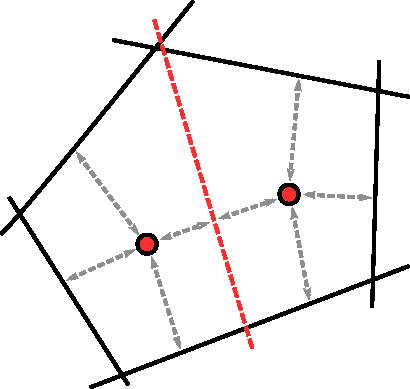
\includegraphics[width=16em]{setmargin}
    \end{center}
    \caption{\label{fig:setmargin} Intuition.}
\end{figure}

\paragraph{MILP Formulation.} This initial formulation is problematic, as
Eq~\ref{eq:wxconstr} involves quadratic terms. Here we show how to reformulate
the problem as a mixed integer linear program (MILP). Our goal is to replace
Eq~\ref{eq:wxconstr} with a set of linear constraints through a suitable
variable transformation.

In order to do so, we introduce a set of fresh variables $p^{i,j}_z$ for every
$i,j\in[k]$ and $z\in[n]$. Each $p^{i,j}_z$ is enforced to be equal to the
product $w^{i}_z x^{i}_z$ through additional constraints. Assuming for the
time being these constraints to be already in place, we rewrite the fourth
component of the objective function in terms of the new variables as:
%
$$ \gamma \sum_{i=1}^k \sum_{z=1}^n p^{i,i}_z $$
%
and, similarly, Eq~\ref{eq:wxconstr} as:
%
\[ \forall \; i, j \in [k], i \neq j \;.\; \sum_{z=1}^n p^{i,i}_z - p^{i,j}_z \ge M \label{eq:pxconstr} \]
%
The fact that $p^{i,j}_z$ takes the value $w^{i}_z x^{i}_z$ is achieved by
setting the following additional constraints. We distinguish between two cases:
(i) $p^{i,i}_z$, and (ii) $p^{i,j}_z$ for $i \ne j$.  Recall that we are
maximizing the margin $M$. Now, due to Eq~\ref{eq:pxconstr}, the optimizer will
try to keep $p^{i,i}_z$ as large as possible and $p^{i,j}_z$ as small as
possible. \stefano{this is not necessarily the case, $M$ is bounded by the
$y$'s as well.}

(Case i) We add an explicit upper bound:
%
$$ p^{i,i}_z \le \min \{ w_\text{max} x^{i}_z, w^{i}_z \} $$
%
where $w_\text{max}$ is a sufficiently large constant.
On one hand, if $x^i_z = 0$ the product $w^i_z x^i_z$ evaluates to $0$, and so does
$p^{i,i}_z \le w_\text{max} x^{i}_z = 0$. On the other hand, if $x^i_z=1$
then the product $w^i_z x^i_z$ amounts to $w^i_z$. In this case, the upper
bound evaluates to $\min \{ w_\text{max}, w^{i}_z \}$. By taking a sufficiently
large constant $w_\text{max}$ (e.g. $w_\text{max} := \max_z w^\top_z$) the upper bound
boils down to $w^i_z$. Since $p^{i,i}_z$ is being maximized, it will attain the
upper bound, and thus evaluate to $w^i_z x^i_z$.

(Case ii) We add an explicit lower bound:
%
$$ p^{i,j}_z \ge \max \{ 0, w^{i}_z - w_\text{max}(1 - x^{j}_z) \} $$
%
If $x^i_z = 1$ the lower bound simplifies to $\max \{ 0, w^{i}_z \} = w^{i}_z$,
due to the non-negativity of $w^i_z$, as expected. Otherwise, if $x^i_z = 0$
then the lower bound becomes $\max \{ 0, w^{i}_z - w_\text{max} \}$, where
the second term is at most $0$. Since $p^{i,j}_z$ is being minimized, in both
cases it will attain the lower bound, and hence equate to $w^i_z x^i_z$.

Substituting the above MILP constraints into the original optimization problem,
we obtain:
{\footnotesize
\begin{align}
    \max_{M, W, X}
        & \;\; M - \alpha \sum_{i=1}^k \| \veps^{i} \|_1 - \beta \sum_{i=1}^k \| \vw^{i} \|_1 + \gamma \sum_{i=1}^k \sum_{z=1}^n p^{i,i}_z
        \nonumber
    \\
    \text{s.t.}
        & \;\; \forall \; i \in [k], \forall \; h \in [n] \nonumber
    \\
        & \;\; \qquad \langle \vw^{i}, \vy^{h}_+ - \vy^{h}_- \rangle \ge M - \varepsilon^{i}_h \nonumber
    \\
        & \;\; \forall \; i, j \in [k], i \neq j \;.\; \sum_{z=1}^n p^{i,i}_z - p^{i,j}_z \ge M
    \\
        & \;\; \forall \; i \in [k], \forall \; z \in [n] \nonumber
    \\
        & \;\; \qquad p^{i,i}_z \le \min \{ w_\text{max} x^{i}_z, w^{i}_z \}
    \\
        & \;\; \forall \; i, j \in [k], i \neq j \nonumber
    \\
        & \;\; \qquad p^{i,j}_z \ge \max \{ 0, w^{i}_z - w_\text{max}(1 - x^{j}_z) \}
    \\
        & \;\; \forall \; i \in [k] \;.\; \vw^\bot \le \vw^{i} \le \vw^\top \nonumber
    \\
        & \;\; \forall \; i \in [k] \;.\; \vx^{i} \in \calX_{\text{feasible}} \nonumber
    \\
        & \;\; \forall \; i \in [k] \;.\; \veps^{i}_h \ge 0 \nonumber
    \\
        & \;\; M \ge 0 \nonumber
\end{align}

}

\subsection{Set-wise Preference Elicitation}

\stefano{WRITEME}

See Algorithm~\ref{alg:setmargin}.

\begin{algorithm}
{\footnotesize
\begin{algorithmic}[1]
    \Procedure{SetMargin}{$k, \alpha, \beta, \gamma, T$}
        \State $\calQ \gets \emptyset$
        \For{$t = 1, \ldots, T$}
            \State \{$\vw^{i}, \vx^{i}\}_{i=1}^k \gets \text{{\sc Solve}}(\calQ, k, \alpha, \beta, \gamma)$
            \For{$\vx^{i},\vx^{j} \in \{ \vx^{1}, \ldots, \vx^{k} \} \; \text{{\bf s.t.}} \; i < j$}
                \State $\calQ \gets \calQ \cup \text{{\sc QueryUser}}(\vx^{i},\vx^{j})$
            \EndFor
        \EndFor
        \State $\vw^*, \vx^* \gets \text{{\sc Solve}}(\calQ, 1, \alpha, \beta, \gamma)$
        \State ${\bf return}\; \vw^*, \vx^*$
    \EndProcedure
\end{algorithmic}
}
\caption{\label{alg:setmargin} The {\sc SetMargin} algorithm. Here $k$ is the
set size, $\alpha,\beta,\gamma$ are the hyperparameters, and $T$ is the maximum
number of iterations. The values of $\calX_\text{feasible}$, $\vw^\top$ and
$\vw^\bot$ are left implicit.}
\end{algorithm}

\subsection{Query Strategy}
\label{sec:querystrategy}

\stefano{WRITEME}

\paragraph{Generalization to real variables.} \stefano{WRITEME}

\section{Experiments}

In this section we provide an experimental evaluation of the {\sc SetMargin}
algorithm. We compare the against two strong Bayesian baselines:
\cite{guo2010real} and \cite{viappiani2010optimal}.


In all experiments we use an internal cross-validation procedure to update the
hyperparameters $\alpha$, $\beta$, and $\gamma$ after every 5 iterations. The
hyperparameters are chosen as to maximize the ranking loss over the user
answers collected so far. $\alpha$ is taken in $\{100, 10, 1\}$,
while $\beta$ and $\gamma$ are taken in $\{100, 10, 1, 0.1, 0\}$. Note that
$\beta=0$ implies that the weight vector is not regularized, nor sparse, while
$\gamma=0$ implies that the absolute quality of the configurations is ignored.
\stefano{is this desirable?}

\paragraph{Synthetic Dataset.} As a first test, we evaluated the performance
of the three methods on a synthetic dataset, where all configurations

We ran all methods on $20$ different users. The hidden, true weight vectors
were the same for all three methods.

\stefano{plot average utility loss at the increase of dataset size}

\stefano{plot average runtime at the increase of dataset size}

\stefano{comment on usefulness of sparse weights}

\stefano{what about an experiment with Horn constraints?}

\paragraph{Constructive Dataset.} \stefano{WRITEME}

- PC dataset without costs

- PC dataset with costs

\section{Conclusion}

WRITEME

\section*{Acknowledgments}

WRITEME

\bibliographystyle{named}
\bibliography{ijcai16}

\end{document}
